% universal settings
\documentclass[smalldemyvopaper,11pt,twoside,onecolumn,openright,extrafontsizes]{memoir}
\usepackage[utf8x]{inputenc}
\usepackage[T1]{fontenc}
%\usepackage[osf]{Alegreya,AlegreyaSans}
\usepackage[osf]{ebgaramond}

%\usepackage[cmintegrals,cmbraces]{newtxmath}
%\usepackage{ebgaramond-maths}
%\usepackage{ebgaramond}
%\usepackage{garamondlibre}

\usepackage{pgffor}
\usepackage{babyloniannum}

% PACKAGE DEFINITION
% typographical packages
\usepackage{microtype} % for micro-typographical adjustments
\usepackage{setspace} % for line spacing
\usepackage{lettrine} % for drop caps and awesome chapter beginnings
\usepackage{titlesec} % for manipulation of chapter titles

% for placeholder text
\usepackage{lipsum} % to generate Lorem Ipsum

% other
\usepackage{calc}
\usepackage{hologo}
\usepackage[hidelinks]{hyperref}
%\usepackage{showframe}

% PHYSICAL DOCUMENT SETUP
% media settings
\setstocksize{8.5in}{5.675in}
\settrimmedsize{8.5in}{5.5in}{*}
\setbinding{0.175in}
\setlrmarginsandblock{0.611in}{1.222in}{*}
\setulmarginsandblock{0.722in}{1.545in}{*}


% defining the title and the author
%\title{\LaTeX{} ePub Template}
%\title{\textsc{How I Started to Love {\fontfamily{cmr}\selectfont\LaTeX{}}}}
\title{Wadborough forest}
\author{John-John Markstedt}
\newcommand{\ISBN}{0-000-00000-2}
\newcommand{\press}{}


% custom second title page
\makeatletter

\let\@chapterfootnote\@empty%
\newcommand{\chapterfootnote}[1]{\gdef\@chapterfootnote{#1}}%
\newcommand{\thechapendfootnote}{{%
		\renewcommand{\thefootnote}{\fnsymbol{footnote}}%
		\ifx\@empty\@chapterfootnote\else
		\footnotetext[1]{\@chapterfootnote}%
		\fi}%
	\let\@chapterfootnote\@empty}%
\newcommand{\chapendfootnote}{%
	\let\oldchapter\chapter%
	\renewcommand{\chapter}{%
		\ifnum\value{chapter}<1\else\thechapendfootnote\fi%
		\oldchapter%
	}%
}

\newcommand*\halftitlepage{\begingroup % Misericords, T&H p 153
  \setlength\drop{0.1\textheight}
  \begin{center}
  \vspace*{\drop}
  \rule{\textwidth}{0in}\par
  {\Large\textsc\thetitle   \\[1in]\par}
  \rule{\textwidth}{0in}\par
  \vfill
  \end{center}
\endgroup}
\makeatother

% custom title page
\thispagestyle{empty}
\makeatletter
\newlength\drop
\newcommand*\titleM{\begingroup % Misericords, T&H p 153
  \setlength\drop{0.15\textheight}
  \begin{center}
  \vspace*{\drop}
  \rule{\textwidth}{0in}\par
  {\HUGE\textsc\thetitle \\[1in]\par}
  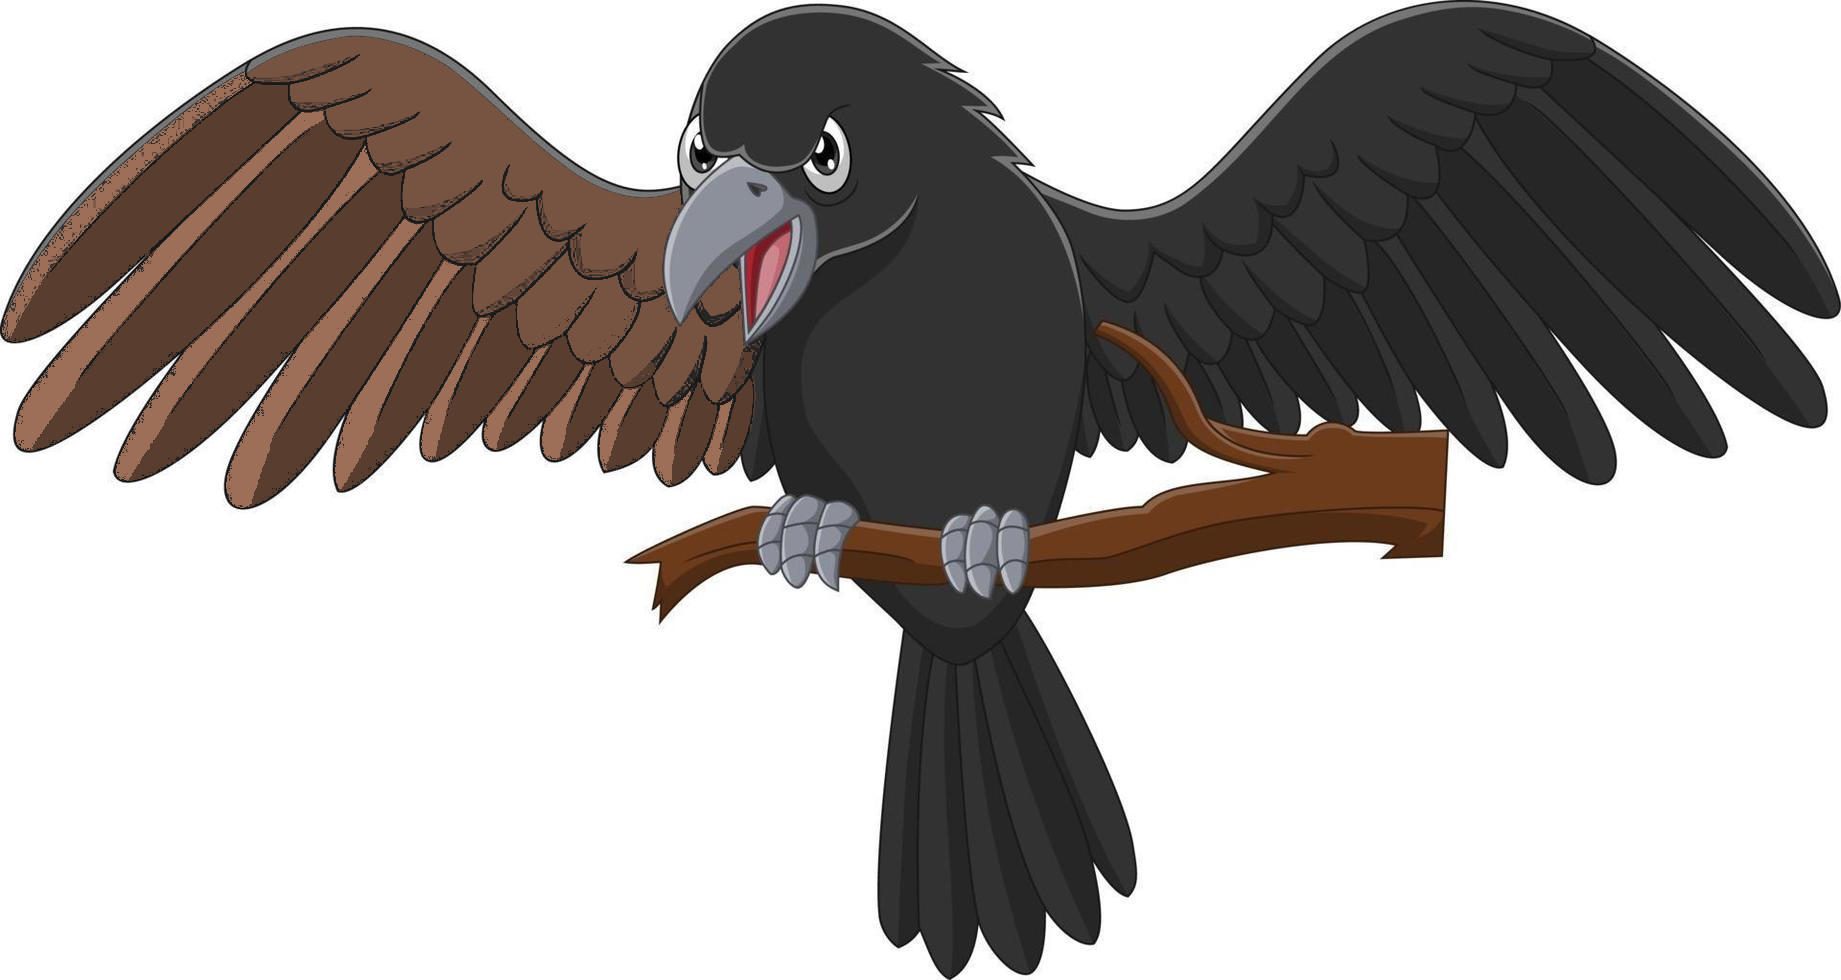
\includegraphics[width=250pt]{eaglewing.png}
  \rule{\textwidth}{0in}\par
  {\Large\textit\theauthor\par}
  \vfill
  {\Large\scshape\press}
  \end{center}
\endgroup}
\makeatother

% chapter title manipulation
% padding with zero
\renewcommand*\thechapter{\ifnum\value{chapter}<10 \fi \babylonian{chapter}}

\renewcommand*{\thepage}{\footnotesize\babylonian{page}}


% chapter title display
\titleformat
{\chapter}
[display]
{\vspace{-2cm}\normalfont\scshape\huge}
{\HUGE\thechapter\centering}
{0pt}
{\vspace{8pt}\centering}[\vspace{22pt}]

% typographical settings for the body text
\setlength{\parskip}{0em}
\linespread{1.09}

% HEADER AND FOOTER MANIPULATION
  % for normal pages
  \nouppercaseheads
  \headsep = 0.16in
  \makepagestyle{mystyle} 
  \setlength{\headwidth}{\dimexpr\textwidth+\marginparsep+\marginparwidth\relax}
  \makerunningwidth{mystyle}{\headwidth}
  \makeevenhead{mystyle}{}{\textsf{\scriptsize\scshape\thetitle}}{}
  \makeoddhead{mystyle}{}{\textsf{\scriptsize\scshape\leftmark}}{}
  \makeevenfoot{mystyle}{}{\textsf{\scriptsize\thepage}}{}
  \makeoddfoot{mystyle}{}{\textsf{\scriptsize\thepage}}{}
  \makeatletter
  \makepsmarks{mystyle}{%
  \createmark{chapter}{left}{nonumber}{\@chapapp\ }{.\ }}
  \makeatother
  % for pages where chapters begin
  \makepagestyle{plain}
  \makerunningwidth{plain}{\headwidth}
  \makeevenfoot{plain}{}{}{}
  \makeoddfoot{plain}{}{}{}
  \pagestyle{mystyle}
% END HEADER AND FOOTER MANIPULATION

% table of contents customisation
\renewcommand\contentsname{\normalfont\scshape Contents}
\renewcommand\cftchapterfont{\normalfont}
\renewcommand{\cftchapterpagefont}{\normalfont}
\renewcommand{\printtoctitle}{\centering\Huge}

% layout check and fix
\checkandfixthelayout
\fixpdflayout

% BEGIN THE DOCUMENT
\begin{document}
	
\newenvironment{localsize}[1]
{%
	\let\orignewcommand\newcommand
	\let\newcommand\renewcommand
	\makeatletter
	\input{bk#1.clo}%
	\makeatother
	\let\newcommand\orignewcommand
}	
	
\pagestyle{empty}
% the half title page
%\halftitlepage
\cleardoublepage
% the title page
\titleM
\clearpage
% copyright page
\noindent{\small{This novel is entirely a work of fiction. The names, characters and incidents portrayed in it are the product of the author's imagination. Any resemblance to actual persons, living or dead, or events or localities is entirely coincidental. \par\vfill\noindent Revision 1 Edit.\space\today\\ISBN\space\ISBN\\\copyright\space\theauthor. All rights reserved.\par\vfill\noindent\theauthor\space asserts the moral right to be identified as the author of this work. All rights reserved in all media. No part of this publication may be reproduced, stored in a retrieval system, or transmitted, in any form, or by any means, electronic, mechanical, photocopying, recording or otherwise, without the prior written permission of the author and/or the publisher.\par}}
\clearpage

% dedication

%\itshape{\noindent{Dedicated to my all {\fontfamily{cmr}\selectfont\LaTeX{}} users.}}



% begin front matter
\frontmatter
\pagestyle{mystyle}
% preface
\chapter*{Preface}

This is the first out of two external revisions. So---although, I'd appreciate comments regarding grammatical errors, sentence structures and formulations---the focus is intended to be on the consistency of the story, the flow of the writing, the entertainment to the reader, and, most notably, the quality and feasibility of the book.

There will be, if this first one goes well, a second revision, where the focus will solely be on the language.

I've made an effort use British spelling and British words where there are multiple possibilities. E.g. brook over creek, autumn over fall, rubbish over trash.

Notably I've chosen to use whilst and amongst as the conjunction, preposition, adverb, and while solely for the verb. Similarly, I've chosen to use the somewhat increasingly archaic verb form of but. \\

This story is a satire; therefore, it touches on many ideas and references that is not entirely self contained within this book. It is my wish that the story is in itself self contained(in the same way Animal farm is self contained, albeit very boring if no association to the real world is allowed). However, much of the fun(or value) in reading it comes with the understanding of symbolism and the mockery within it. 
As part of this first revision, I've noted every outside reference(those that are intentional at least) made in this work. I do not want to rely on obscure knowledge of trivia however, and those references should not harm the experience of reading---if so, they should be removed. Please note every reference you are able to find---even the ones that are almost too obvious.
I've divided every outside reference in to three categories.

First category: Contains very few but obvious references that I think should be known by 80\% of the populace aged 18 or over. Failing to understand these would make a really dull read.
Second category: The category that contains
 most references made, they are not necessary to read the story but understanding a few of them would certainly increase the joy of this book.
 
Third category: This category contains all obscure references. They should be completely passed over with no hiccup, i.e. you'd never guess it's an reference if not told so. Some of these require some deduction, and I hope that even if they're found, It's not obvious that I put it there intentionally.

Perhaps unnecessary remark 1: the chapter quotes are carefully picked and are all relevant to the chapter's text.

Perhaps unnecessary remark 2: the character names are carefully picked and are all relevant to the story(albeit some more than others).\\[1cm]
Chapters:\\
1: Intro\\
2: Build up\\
3: Build up\\
4: Pay off\\
5: Neither\\
6: Pay off\\
7: Build up\\
8: Build up\\
9: Pay off\\
10: Neither\\
11: Neither\\
12: Pay off\\

Characters:\\[1cm]
Introduced Chapter 2:\\[0.1cm]
Kraerion,
Aequitus\\[0.1cm]
Mentioned:\\[0.1cm]
Br'er Rabbit,
Ongenþeow,
Pietus,
Veritas,
Cinnamon\\[1cm]
Chapter 1\\[1cm]
c3: Darwin quote, hints to a tertiary theme of the book: [redacted].\\
c3: published in 1859, it fits perfect being ruffly 10 years before la belle epoque.\\
cX: I'm a fan of Darwin's work\\
c2: 'Natural checks and balances': a very darwinian sentence.\\
c3: Locks of gold --- Goldilock: both: https://en.wikipedia.org/wiki/Goldilocks\_economy, and https://en.wikipedia.org/wiki/Circumstellar\_habitable\_zone\\
c3: The beautiful era: La Belle Époque: https://en.wikipedia.org/wiki/Belle\_Epoque\\
chapter 2 \\
will be filled after you've read it.

Enjoy!


% acknowledgements
%\chapter*{Acknowledgements}

% table of contents
\clearpage
\tableofcontents*

\clearpage

%\pagenumbering{roman}

%\vspace*{4.3cm}
%\begin{center}
%	\begin{localsize}{10}
%		In memory of Richard Adams\\
%		\begin{quote}
%			“My heart has joined the Thousand, for my friend stopped running today.”
%			\begin{flushright}1920 -- 2016\end{flushright}
%		\end{quote} 
%	\end{localsize}
%	\vspace{1cm}
	
%\end{center}

\clearpage

\vspace*{4.3cm}
\begin{localsize}{10}
  \begin{quote}
    “Some people talk to animals. Not many listen though. That's the problem.”
    \begin{flushright}- A.A Milne \end{flushright}
  \end{quote} 
\end{localsize}
\vspace{1cm}

% begin main matter

%“The struggle of man against power is the struggle of memory against forgetting”

%If the misery of the poor be caused not by the laws of nature, but by our institutions, great is our sin.

%The last capitalist we hang shall be the one who sold us the rope.

%Money is a formal token of delayed reciprocal altruism.

%To know that we know what we know, and to know that we do not know what we do not know, that is true knowledge. 

% under suitable conditions, cooperation can indeed emerge in a world of egoists without central authority. Robert Axelrod

% Thus, under suitable conditions, cooperation based upon reprocity proves stable in the biological world.

% “The hardest thing to explain is the glaringly evident which everybody has decided not to see.” ayn rand

% “In man's struggle against the world, bet on the world.” Franz kafka
% “I dream of a grave, deep and narrow, where we could clasp each other in our arms as with clamps, and I would hide my face in you and you would hide your face in me, and nobody would ever see us any more” Kafka

% “If a man does not keep pace with his companions, perhaps it is because he hears a different drummer. Let him step to the music he hears, however measured or far away.” - Henry David Thoreau

%“Communism is not love. Communism is a hammer which we use to crush the enemy.” - Mao Zedong

%"To read too many books is harmful. " - Mao Zedong
% “The more I read, the more I acquire, the more certain I am that I know nothing.” - Voltaire

%“The average man is both better informed and less corruptible in the decisions he makes as a consumer than as a voter at political elections.” - Ludwig von Mises

% “'Emergencies' have always been the pretext on which the safeguards of individual liberty have eroded.” - Friedrich August von Hayek

% “I have never made but one prayer to God, a very short one: Oh Lord, make my enemies ridiculous. And God granted it." - Voltaire

% “Until they become conscious they will never rebel, and until after they have rebelled they cannot become conscious.”  Orwell

% “The society that puts equality before freedom will end up with neither. The society that puts freedom before equality will end up with a great measure of both” Friedman

% “Hell is truth seen too late.” 


% “Virtue is more to be feared than vice, because its excesses are not subject to the regulation of conscience.” Smith

\mainmatter
%\pagenumbering{hexadecimal}
%\renewcommand*{\thepage}{\hexadecimal{page}}


\chapter{Deordination}
\vspace{-1.3cm}
\begin{localsize}{10}
	\begin{quote}
		"Man selects only for his own good; Nature only for that of the being which she tends."
		\begin{flushright}- Charles Darwin\end{flushright}
	\end{quote} 
\end{localsize}
\vspace{1cm}

The Wadborough forest is a peculiar collection of trees; it's shaped by an improbable set of circumstances, setting the preconditions of this unlikely tale you're about to read. % shaped by an equally peculiar set of circumstance; setting the unique condition of this unlikely tale.

The forest has stood where it now stands for millennia, but surrounded by other trees and part of a much larger forest: it did not crave attention, nor require distinction by name. With the ever increasing sophistication---and population grow- th---of the main British isle, most trees were cut down for timber, and the woodlands were slowly turned to grazed meadows and tiled farmlands. The trees near the little village of Wadborough would most certainly meet the same fate, if it wasn't for a growing posh ritual of high British society. The Duke of Worcestershire---lest he lose pace with his peers---began importing pheasants to be hunted by his guests and his more distinguished subjects. He thus proclaimed that the trees near the Wadborough village would never be cut down, and ever solely be allocated to the hunting of game. These trees became the Wadborough forest---standing tall and alone in the wild ocean of fields.

Pheasants are clumsy birds---used to roam the Asian steps undisturbed by predators---and found it difficult to survive in the forest. To protect their precious game: the Duke's men drove, over the years, all major predators out of the region. The red fox was first to go(to the chickens' rejoice) as they seemed almost offended by the ease of hunting pheasants. The weasel family: the stoat, the wolverine, and the mink; followed shortly thereafter. The badgers were also hunted, but they soon understood that the pheasants were off limit and began to ignore the foreign bird; thus, a few badgers remained alive. As with all human interventions: they're seldom without unforeseen consequences; the rodent population boomed; which, incidentally attracted more birds of prey to the region. These birds---mostly consisting of various hawks and species of owls---did not danger the life of pheasants; however, they possessed another threat entirely. The ornithologists of the time had a fierce reputation of enacting conservation legislation; the rumor of the birds broad prevalence reached the group and soon they took interest in the forest. The Duke thus had a choice: spare the birds and risk the ornithologists' influence, or kill them and risk the outbreak of rodents; he chose the latter. The rodents did explode in numbers, but they did not carry disease with them, nor overrun the neighbouring fields and the Wadborough village. As a matter of fact---the rodents did not at all conform to the behaviours so often attributed to them. No one could explain why.

Eventually the time of serfdom met its end; and the society slowly morphed into something approaching the appearance of a representative democracy. Ownership of land transferred from lords and ladies to the establish municipalities, and so too did the ownership of the Wadborough forest. Although hunting remains a tradition of the well-off, its clientele slowly shifted to in time mostly consist of ordinary rural villagers.   
Innovations in agriculture and growing manufacturing greatly shifted the populace from rural to urban. The growing cities lost touch with the rural arts. Hunting---especially when performed as sport as it is with game---became viewed as cruel and barbaric. The urban population greatly outnumbered its rural counterpart in voting power; activists rallied and tallied support---the Bill of The Wildlife Preservation Act soon passed through the county of Worcestershire; which, conveniently holds the legislative power in Wadborough. The Act contained many a paragraph, but only one concerned the Hunters of Wadborough. 

\begin{localsize}{10}
	\begin{quote}
		'A person shall not hunt game birds including but not limited to the Common Pheasant, Grouse, Goose, Turkey, Duck or Pigeon by means of firearm, or any form of projectile, unless bread in captivity under permission from a state licensed breeder(§95b). A person guilty of offense under this Act shall be liable on summary conviction to a fine not exceeding 5.000 pound sterling.'
		\begin{flushright}- §68, The Wildlife Preservation Act\end{flushright}
	\end{quote} 
\end{localsize}
 
The Act angered the villagers; "what does city folk know of hunting!?" could be heard at the local drinking holes. Wild conspiracies was liberally spread along with wild guesses on the probabilities of actually getting caught. To the villagers dismay, the city clerks had foreseen their unwillingness to abide by the new law and were ruthlessly prepared to hand out many a salted fine during the first year of the bill's passing. 

And so it came to be that the forest of Wadborough was free of both predator and man alike---undisturbed by the natural checks and balances that keeps the order of things. Even the locks of gold couldn't compare to the beautiful era that would follow.



\chapter{Doubt}

\vspace{-1.3cm}
\begin{localsize}{10}
	\begin{quote}
		“I have never made but one prayer to God, a very short one: Oh Lord, make my enemies ridiculous. And God granted it."
		\begin{flushright}- Voltaire \end{flushright}
	\end{quote}
\end{localsize}
\vspace{1cm}


"One day is today---", Kraerion whispered to himself as his tired eyes slowly widened to an open state. The chimpunk had woke---like all mornings---to a loud unpleasant banging sound, echoing around the run outside the comforts of his small burrow. The sound carried with it the news of a new day, and with it: the message that all who wanted a day's pay ought to drag themselves to the great hall, the Aorta, presently. The frowsty air this deep underground usually made him rise as soon as he woke---to seek a more pleasant ambiance---but today he lingered in thoughts.

"One day is today.", he repeated, to reassure himself and still his doubts, as if repeating the words would make them more true. The power of inertia is strong; Kraerion full well knew of its insidious nature: that tomorrow and never were but equal measurements of eternity. He had longed---even dreamed---for this day to come for as long as he could remember; so he wondered why---now when the day was finally here---he had so suddenly lost his strong convictions.

Chipmunks may be genetically poised for a life underground, but not the chipmunk Kraerion. Even as a little kitten, he had loathed their exists: the damp runs and burrows, the second-hand air, the ever present darkness, and about everything else underground just by association. He hated---as only an adolescent can hate---that which most of his peers called home.
Instead, he wished for a strong wind in his fur, sunlight that uncovered all the beauty that is Nature, but most of all the chaotic buzzing of life above, that so contrasts the routines down below. He yearned to run the branches of trees, not the ever branching network of runs dug in the forest soil. His father had many a time japed that his son was born more a squirrel than chipmunk---and he had not been wrong. When he was younger, he had stated that one day he was going to live amongst the trees, but received feedback which would otherwise only be appropriate after a well executed joke.

Kraerion eventually mustered the will to rise from his moss coated bed. He went over to a corner of his burrow and began scratching away at the dirt.

"Good, still here.", he confirmed anxiously, as the felt the steel of seven steel screw-nuts---which would surely appear beautiful in the sunlight---laying before him. He covered them up again and left his burrow into the run, and followed its twists and turns until it widened into a great hall: the Aorta. It was dug under a great willow; its massive network of roots---intertwined with the walls and ceiling---supported the weight of the dirt and kept it from caving in.\\

Since the time of Man, the forest had steadily increased its economic output. One of the  contributing factors was the increased specialization of its inhabitants. Whilst many a specie have some certain advantage in the gathering of some specific type of feed, none is as great a carrier than that of the chipmunk. In their elastic cheeks, they are able to carry loads of feed---and other goods for that matter---efficiently around the forest; their small size and great numbers gave the operation a granularity to it, which made it difficult for larger and stronger animals like the roebuck to compete. When other animals began to hire them for their service, they began to expand their network of tunnels and runs to cover whole forest---connecting all its major hubs. Therefor---every morning---the chipmunks gathered in the Aorta to share news and plan the day ahead.

Most chipmunks were already present when Kraerion entered. 

"One day is today.", he thought again, as he headed towards his usual spot in the front. But he hesitated suddenly and reconsidered; instead, he decided to begin his new life with breaking this habit and found a place in the back.\\

The murmur of conversation disappeared in an instance when an old chipmunk appeared in the Aorta. His name was Aequitus and was the chief chipmunk, gray spots of fur spoke of his age, yet his features were easy on the eye and he bore his age proudly. Everyone knew the chief and saw him as something akin to a revered hero. When he was but a kitten, he'd taken interest in the chipmunks' livelihood and noticed irregularities in their billings; after some further deliberation with his friend Br'er Rabbit, he realized that they could likely double their prices with little to no churn. He put forth the motion to the then chief chipmunk, who surprisingly listened to the youngster and approved it. When their income subsequently increased, he was very vocal about its occurrence, and made it impossible for the chief chipmunk not to pass it forward to the chipmunks' daily wage.

When Aequitus a few years later became unanimously chosen as the next chief, he took it a step further. He transformed the chipmunks' enterprise to a sort of cooperative, with bylaws dictating that a fixed percentage of the total revenue would be earmarked for workers' wages. As well as other rules limiting the influence of his own office---not only for himself but setting the precedence for his eventual replacements. 

Together with Br'er Rabbit---who had by then become the implicit leader of the rabbits---and with the help of the by  then Glade of Representatives Twig Ongenþeow, he started the Winter Fund. A collective fund that functions similar to that of human insurance: its members contributes feed during the spring, summer, and autumn as a premium; members that find themselves short during the winter may then make a claim and receive feed to sustain them until winter's end. % Dearth

A cynic human might proclaim the flaw in this scheme, that an animal might take advantage of it by wasting his wage and making a claim every winter---but he forgets two things: most animals can't count; and although possible, making a claim is very stigmatized, and that most animals would rather starve than to broadcast their destitution. Aequitus also---being a co-founder of the fund---made sure that all the work related to the logistics---moving and storing of the feed deep underground, where the soil is grainy, cold, and preserves the feed from pest and rot, and hidden from prying thieves---went to the chipmunks---further boosting the demand for their services.

The fund was a great success; winter deaths decreased drastically the first year, and then slowly year after year. The chipmunks got a more steady stream of sophisticated work from the fund and thus means for a better life. For all the contributions Aequitus made, none could match the feeling he instilled in every chipmunk: the intangible sense of worth; the standing the brought them to in the forest; and the care he fostered between chipmunks by treating them all as equals.\\

When Aequitus reached the front of the Aorta, he turned and faced the scurry.

"Before we go through today's agenda, I have news---both good and bad.", he began, "And, as you may not be able to appreciate the good in anticipation of bad, I'll begin with the bad.", he took a tactful pause, as anyone with his level of experience would in this situation.

"The eastbound run collapsed late last evening; we're completely cut off from the eastern part of the forest. Therefor, the deliveries to the rabbits' hill must be postponed."

"Why did it collapse?", Aequitus younger brother Pietus asked, who stood at his regular place just right of his brother.

"Well---", Aequitus dragged, "a pheasant went chasing a maggot again and crossed above the shallow no-zone."

"Again!?", Pietus cried, not hiding his contempt, "Did the pheasants not promise to be more careful---that last time would be the last? Will they honour our agreement and pay for the damages?"

"They did indeed. As you all know, the pheasants are not the most organized of animals and will only blame each other if we make a claim for damages. We may bring it to the Glade, but what---other than appearing petty---would we gain? Little and less, I'm afraid. Nevertheless, I want you, Pietus, to go to the moles and have them dig a deeper eastbound run this time---that is, at least, a factor we can affect."
"I'll do it.", Pietus responded, "But send someone else to the moles next time---they don't even speak our language..." %the common tongue.

"Nā, hēo seċġaþ þone ealda sprǣċe. It is we that don't speak theirs.", Aequitus paused, waiting to see if Pietus had a response. When his brother only mumbled something inaudible, he continued.

"I'll make sure Br'er and the rabbits get the news of this postponement personally. As for the good news, the rumors going around are true: the Glade have decided to institute a 2\% tax on all Forest shipments. It's only a temporary experiment with us as the pilot service."

"How is this good news?", Veritas squeaked, a tiny runt of a chipmunk who were also standing in the front close to Aequitus.

"Two reasons: firstly, the funds are marked as aid for destitute animals who can't afford the Winter Fund, and we'll surely get the contract for its operation; secondly, we don't pay for our own services---we're essentially exempt!"

"No! That's not how it works.", Veritas snapped angrily, "this will force an increase in our prices---hurt our margins; to only burden one industry, and ours at that---it's... it's incredibly unfair."

"Enough.", Aequitus grumbled, "That's enough, this is neither the place nor time, we may discuss this later in private."

Veritas did not answer, but she turned her head sideways---showing everyone her disdain.

The old chipmunk moved on to the day's normal agenda, dishing out more routinely orders before dismissing his workforce. However, his eyes were fixed on Kraerion---the dismissal did not apply to him. When the last chipmunk had left the Aorta, he began to speak.

"Kraerion---", he said.

"Father.", Kraerion responded, equally enthusiastic.

"It's true then, hiding in the back like that; you're actually leaving what we worked so hard to create?"

"What you created you mean? You cannot pretend this is news---I've been more than forthcoming with my intention to lead a different life. You of all chipmunks should know of my extra shifts to afford this move, and my refusal of the managerial responsibilities you so blatantly pushed on me."

"We all have dreams, Kraerion. I know you might \textit{feel} like a squirrel, but you're not one---I promise you that you'll end up miserable, dearth of resources, and completely alone in a world of wings if you try to live as one.
Dreams are a lesson in growing up: learning how to smother them in favour of what's truly important in this life. And, you'll get other dreams---realistic dreams---like forming a family, building a future for our specie, and contributing to the betterment of the Forest at large."

"I'm sorry---", Kraerion said at length, "but that's not me, and quite frankly, that'll never be me."

"Don't you feel any sense of responsibility? What about your sister Veritas? You expect Pietus and I to go on forever?"

"What about her? She's smarter than us three combined; she could take over tomorrow if you'd only let her."

"You know full well that intelligence isn't everything. You saw how she acted today: she lacks the social conduct to lead other chipmunks."

"Maybe you should have spoken with her before announcing your decision to the whole Aorta?"

"It's not only today and you know it. Never mind. If not for us, then what of you and Cinnamon?"

"Don't", Kraerion said flustered.

"What, you haven't told her!?", Aequitus said truly surprised; he was just about scold his son, but hesitated when he saw Kraerion's face and realized it would be superfluous. Before he had time to say anything more, Kraerion turned around and ran.

Kraerion ran, and he ran, and he kept on running until the pain in his lungs, and muscles, numbed the thoughts that so rudely had occupied his mind.

%\chapter{Dread}

\vspace{-1.3cm}
\begin{localsize}{10}
	\begin{quote}
		"'Emergencies' have always been the pretext on which the safeguards of individual liberty have eroded."
		\begin{flushright}- Friedrich Hayek\end{flushright}
	\end{quote} 
\end{localsize}
\vspace{1cm}

\renewcommand*{\thepage}{\footnotesize \hexadecimal{page}}

Kraerion eventually stopped running; once his emotions cooled off, he felt embarrassed for how he had acted. 

"Well, good riddance---", he thought, "at least I can't go back now. One day is truly today."

The chipmunk returned to his burrow one last time, to fetch his screw nuts and say his goodbyes. He had stood there for a very long time; not knowing how to say farewell, and he somehow felt that the moment required a solemn pause. When he made an attempt to leave, his legs refused; he felt an annoyance for his own nostalgia. Life underground was all he had known; nothing would ever be the same.

When he exited the networks of runs through the exit known as the Northwestern Arteriole, a large woodpecker were already waiting for him. His name was Redrill, and he had an especially pronounced red crest. Woodpeckers made excellent woodworkers, but most of them worked in small teams and only took on larger construction projects. But not Redrill, he was a loner and preferred to work alone and had hence accepted Kraerion's rather unorthodox request. The seven screw-nuts he had fetched were awkwardly wrapped around his front legs, and caught the sunlight and glimmered harmoniously. 

\renewcommand*{\thepage}{\footnotesize \arabic{page}}

"You're really sure about this?", Redrill asked.

"Yes!", Kraerion answered, maybe a bit too quickly, as if he was caught with his paw down a honey pot, "I---I mean, I've never been more sure."

"Don't worry,", Redrill chuckled amused, "I won't argue with the hand that feeds me. I see you've brought payment."

"Well, only one is for you though. Better get going."

The woodpecker smiled, nodded, and unfolded his wings and set off north with Kraerion---with all his might---trying to keep up the pace through the thick undergrowth.\\

The Wadborough villagers---in a time before environmental concerns---dumped much of their \textit{undesirables} in the forest. Everyone denied it---of course---yet batteries, plastics, electronics, and everything else one can imagine found itself in every nook and cranny of the forest floor. Even a run down car or two occasionally joined the detritus. Most animals---after a good whiff---would not bother with these alien contraptions. But, in a magpie a curiosity grew; soon, he conjectured: these objects of Men may teach a thing or two! The magpie began to take them apart; study their intricate design and their innate structures. He felt an unnatural compulsion towards to the weird family of human fasteners: the screw nuts. Death may be the mother of all beauty, yet these imperishable hexagons of cast steel were of different kind. Sun rays bouncing off their plain silver surfaces caught the magpie in awe; the beauty consumed him, and he eventually took to hoarding. The desire for these little things spread like wildfire; first amongst the magpies and the other birds in the crow family, but soon all animals had taken a fancy to them---a treasured commodity was born. But it wasn't like any other commodity: it endured where blueberries rot, it was portable where trees stood firm, but most significant was its limited supply---a thing of Man. It couldn't be produced like the spines of a hedgehog's back, nor grown like the acorns of an oak tree. Naturally, the young economy was tired of barter and sought a system to keep better score: an informational instrument to keep track of favours; a fair system of time allocation. And thus, for the first time in the kingdom of animal, go beyond reciprocal altruism---transcend death---and let a money be born.  

But to Kraerion, the screw nuts were but a means to an end: to purse life anew. \\

The day was a beautiful one; the sun shone bright on a blue canvas sky with only a few dots of white. His seven screw-nuts around his legs made it difficult to run, and he soon lost sight of Redrill. He did not worry though, the woodpecker would not drop his client for a lousy tempo. His anxious feelings from earlier that morning eased somewhat by the fine weather, like the miraculous cure weather so often can be. 

"What a great day!", he said out loud to no one in particular, "What a shame it would be to have it spent underground."

The sun's rays told of high noon, yet the forest was uncharacteristically quiet. Noon was a time of activity, when the animals left their nests, burrows, lairs, and vocational duties to seek out trade. To buy or sell feed; to offer or acquire service. Anything imaginable were up for sale: a blackbird could be hired to sing, a joyride could be enjoyed from the back of a magpie, fresh blueberries---or stolen cabbage from the neighbouring fields---could be bought. Therefor, on any other day, a distant voice in his ears would not have sparked his curiousness. When he reached a clearing in the trees, he leaned back on his hind legs and saw---past the overgrowth---a hedgehog and a robin arguing intensely. He recognized the hedgehog as a acquaintance of his fathers, he knew him as Spinestack, and closed the distance to them.

 "Are you mad?", the robin asked flustered, "Have you completely lost your mind? You know I need more than two measly spines."
 
 "Spines are not weeds you simply pluck from a field of your choosing; they take effort and care to grow.", Spinestack answered calmly, "And these recent---although tragic---events have created a wonderful demand, as you surely understand."
 
 "But... But that's more than trice as expensive than just a couple weeks ago. This is war profiteering! I'm down to my last screw nut; you must understand."

"I mustn't anything.", Spinestack reassured calmly as he saw Kraerion approaching and waved, "I could ask any of your neighbours, who, I'm sure, would find the price both fair and appropriate."

"Wait, hold on,", Kraerion interrupted as he took notice of the small heap of spines, sharp and keen, laying between the two animals, "What do you mean war? And what on earth would you need spines for?"

"Oh haven't you heard!?", the robin squeaked, "It's terrible---\textit{Terr-i-ble} I say: just this morning a nightingale in the same tree as me got her screw nuts stolen. And it's not an isolated incident either, it has happened all over the forest in the last few days. I refuse to sit idle by; we must take up arms and defend ourselves---just like in the tales of the time of Man!"

"Hrmf", Redrill uttered from a twig above the group, seemingly appearing from nowhere, "I heard a few rats have similar complaints earlier this morning, apparently a few of their burrows had been raided. And they are \textit{rats} after all, who dares mess with them?"

"Yes, very sad indeed. Now could you take your discourse elsewhere?", Spinestack said glaring at the two newcomers, "We are conducting serious business here, go waste someone else's time---preferably someone whose time is of less value than mine."

Redrill gave Spinestack a sharp look of disgust, "You've always been more heap than stack, don't you think?", he jested, untucked his wings, and took off. Kraerion had not much choice but to follow.\\

When they reached the silver birch---which was to become Kraerion's home---a fluffy wood pigeon greeted them with a coo. 

"Welcome Kraerion, to our humble and peaceful corner of the Forest.", the pigeon said. His name was Greyhead; this pigeon landlord owned a score of birches and had agree to sell part of one to Kraerion. It was very unusual for one animal to only own part of a tree; most animals paid rent. Kraerion had first been offered to rent, but refused---he was ready for a life free from the burden of economic dependence and thus the need of a steady wage.

"The meter directly above the first twig is yours. I've etched in some markings, you may, of course, measure it yourself."

Kraerion nodded and handed over three of the screw nuts to Greyhead. The pigeon thanked, and having errands elsewhere---excused himself and flew away.

Redrill had received instructions many days ago, and wasted no time consulting Kraerion on what to do. He flew up and landed on the south facing side of the birch and began drilling. The woodpecker's head jerked back and forth, transforming his appearance into a red smear. Kraerion felt very silly when the origins of Redrill's name suddenly dawned on him, he could not believe how he hadn't realized it sooner.

Woodpeckers were not made to carve homes in the trunks of trees. Their strong chisel-like bill and shock-resistant head had slowly been selected by Nature for its ever increasing ability to prey on termites, beetles, and various other larvae dwelling behind bark and wood. But---like most animals---with the rise of a market, their abilities found a vastly greater commercial value elsewhere. And, the woodpeckers found it in carpentry.

Kraerion didn't know how to act whilst Redrill worked. He felt that he would only be in the way if he tried to help, and there was nothing else there he could occupy himself with. He had not stood there long before he was saved by a loud screech from a neighbouring birch.

"Wait here.", Redrill yelled urgingly from up above; he dashed---without hesitation---towards the sound. Kraerion paid no heed; instead, he lunged to the tree and rushed up its trunk. The trunk divided evenly into three large limbs; between them lay a pigeon's nest. He continued up one of the limbs as to look down and see it. Redrill was perched on a branch opposite of Kraerion---they were the first on site. And as pigeons came flying from all directions, they looked down and saw a terrified mother and her three newborn squabs, naked save for their scrawny, near undeveloped down.

"They're gone;", she said despondently, "They're all gone. Oh dear, how will we survive?"

"Won't nest insurance cover it?", a pigeon asked after a long moment of silence.

"No,", another pigeon answered, "theft has not been an issue since the time of Man. Why would anyone even think of including it in coverage?"

"It may yet be rectified, as far as I'm aware, nest insurance has always been implied to cover these kinds of things. I'm sure there's some broad clauses in there that might be stretched to cover this situation.", Greyhead broke in, sighed, "Otherwise, we'll come together and cover it ourselves; solidarity is not yet lost on us. Regardless, the best we can do for now is to give her some room and time to breath, especially by those not yet part of our community."

The insinuation was not lost on either Redrill or Kraerion. Nevertheless, it was a reasonably request, and the two animals vacated the tree.

"We're not particularly popular today.", Redrill muttered jokingly. \\

The moon had long since appeared when Redrill finished his work. The woodpecker sailed down to Kraerion at the foot of the birch.

"I guess I'm done!", he proclaimed, "Are you sure it's deep enough? It's barely more than an entrance."

"Well, you know I can't afford more of your time.", Kraerion answered. "Besides, me teeth should be strong enough to carve out the rest. Take the screw nut before I regret it."

As he handed over one of his screw nuts to the bird, Greyhead appeared again.

"Good evening, excuse my rude remark earlier," the pigeon began, "these are strange times; I hope you don't take it as a reflection of your person."

"No offense taken.", Redrill said whilst Kraerion simply nodded.

"I have some news that might not have reached the two of you yet.", Greyhead continued, "The crows have called for a state of emergency, there's going to be a meeting in the Glade, tomorrow at noon. Thought you'd like to know."

"Okay, thanks.", Redrill said tiredly, yawned, and turned to Kraerion, "It's getting late, are you sleeping here?" 

"Not like I have a choice, the new tenants have most likely already moved in to my old burrow."

"Well then,", the woodpecker said and untucked his wings, prompting Greyhead to do the same. The two birds took off and disappeared into the blissful summer night. Kraerion was left alone with his hollow, his new life, and his ever intruding thoughts. Still unsure if he had made the right decision, he climbed up the tree to his entrance.

"One day was today.", he concluded solemnly. The hollow's floor was still rough and unyielding, but it wasn't the brown soil of a burrow---that was all that mattered. With time, he would widen the hollow, grind the walls and floor sleek, carry up moss and lichen to make a bed, and slowly be able to call it home. That night, he slept uneasy; his body and limbs were heavy and exhausted, yet his mind was unbridled and completely awake. When sleep finally came, it was with an unusual satisfaction that only major life decisions produces---it scared him to know that he'd almost gone a whole life with- 
\newpage
\setcounter{page}{15}
out it.



%\chapter{Diversion}

\vspace{-1.3cm}
\begin{localsize}{10}
	\begin{quote}
		“The struggle of man against power is the struggle of memory against forgetting.”
		\begin{flushright}- Milan Kundera \end{flushright}
	\end{quote} 
\end{localsize}
\vspace{1cm}

%one could argue something similar could be said of those who paid into the winter fund, but they could hide under the name of soldiarity

It may be easy — in places of kind latitudes, or in times of modern comforts — to forget the implications of seasons. The beautiful autumn fires had raged for weeks in the forest's canopy; but now the leaves were falling, a red and orange carpet to invite the forth and final season. 
%Indent
When Man first left the forest generations ago, the animals come together, in the glade of representatives, with a singular purpose in mind: to survive winter. It was an idealistic time, and a crow had uttered the phrase: "No flake of snow shall fall, til every Animal seeth a path to spring.", to a roaring glade - drunk of hope and future prospects, and thenceforth it became known as the crow's law. But, more importantly, it became legend - the story every mother told their kitten, pup, or bunny - and the backbone of moral.
%Indent
No matter how beautiful the law appeared to the first animals, reality seldom bends to beauty; and it had some very real practical limitations.
There were simply too many an animal to listen to them all; but even so, the fraction animals that did speak, had a tendency to refrain from sharing the truth. It requires little difficulty to imagine why an animal would not stand up, in front of the whole forest, and all potential mates, and declare himself incompetent - to advertise his inability to survive the winter without aid. 


%There had long been a custom for the animals to hold an annual meeting the day after the first frost. A moment to finalize the winter preparations, before activity contracted to survival speeds. The autumn colours of fire had fallen from the trees and only rotten leaves remained, like ash, to tell of its tales. The nights grew longer and colder; eventually frost was inevitable. The forest had prospered since the time of men, but winter was still winter - the unprepared would not live to see the spring. 
 
"Craax, hares!", Eaglewing cried tiredly, without his usual tact, as the fifth hour in the glade began, "Thou art next Snowball."

%"Hrm", Snowball uttered as he took a step forward. He looked anything like a snowball, still wearing his brown coat. His beauty was concealed and dormant, but in the next few weeks his fur would transform into a magnificent white coat, the sort of white whom even the snow were jealous of. "Our burrows are filled to the brim with hay. But you all know us, we'll manage to scavenge for food even in the thickest of snow. Our warren will be safe this winter."

"Okey", the hare, who looked nothing like a snowboll, said; but over the coming weeks he would, as would the forest, gain a beautiful coat of white. "Well — yes, we hares are very well prepared. We've estimated that we collectively have 10\% more produce than the year before. And, like the years before, most of us have paid into the Winter Fund as well."

"And dost thou speak for all the hares?", Eaglewing asked, as this was feasible way to comply with the Crow's law.

"Inasmuch as I'm aware."

"If any hare doth not feel spoken for - speaketh now!"

"...so the hare seeth a path to spring." Eaglewing continued when no one spoke and they moved on to the next speaker. And so it went on for many an hour. 

The species in the forest varied greatly in their independence; whilst the hares, rabbits, and chipmunks only required one speaker each, there were just as many on the other side of the spectrum. For instance, all the magpies and roebucks represented themselves, each outbragging the next until it bordered on the ridicoulus. The moles, who did speak their own peculiar language and did seldom partake in forest functions, also lined up the share their story individually; although, they all said a variation of the same sentence: "Ic hæbbe fōda nôg.", and thus went rather quickly.


%The moles, who did speak in their own language and did usually not partake in functions, all lined up to share their status; although, they all said a variation of "Ic hæbbe fōda nôg." and thus went rather quickly. The magpies, and the roebucks, did also all speak, but it did not go as quickly; they seemed to treat it like a bragging con
%Eaglewing seemed content with his answered and continued by calling up the next speaker. 

%Unlike the emergency meeting regarding theft the meeting of the first frost followed a dull routine. 

%Ultimately the animals were individuals against the winter, but their sovereignty ranged over a broad spectrum. On one extreme stood the rabbits who slept in the same hill, pooled digging labor and grazed in large numbers. So only Zefrafal was called upon to speak on the warrens behalf. On the other end were the roebucks who would almost beat each other to death if met during the wrong during the wrong season. Every single buck were thus called upon to speak. A task both time consuming and pointless as bucks were more concerned with boasting their zeal than reveal any concern about any shortages. The rest of species fell in between the two.

%The sun was about to set when only one speaker remained, save for the crows themselves of course. Most animals had stopped listening long ago. The remaining and last to speak was Aequitas of the chipmunks, as was custom since no one knew better than him how much had been transported and stored underground.

The sun was setting by the time all had been spoken for, save for the crows who never spoke. Now only an update of the winter fund remained before the animals could return to their burrows and nests.

"Before I leave the word to Aequitas and the Winter Fund, let me leave this final remark", Eaglewing said, as he regained his tact,

"Every year we gather here, and nigh every year we are better off than the one before. Incrementally quality of life improveth, each year invisible to the eye; nonetheless the generations, in aggegate, since our humble beginnings are visible: the destitute of the savage Animal be now extinct!

Oughtn't we to be content with our progression? Oughtn't we stand in awe - admire our accomplishments? No, we ought to always strive for more - for better; and we have by no means inherited a perfect system. We're at the whims of our market, it ebbs and it flows, but it is never stable - and we suffer for it, when value be erased, jobs be lost, and progress must reset. And even worse: unfairness be innate to markets, its abudance is distributed according to power law — to wit, as the words of Man's God saith: whoever hath, more shall be given; whoever hath not, even that shall be taken away.

No, we oughtn't be content with our progression! And the first step have already been taken, to stabilize market demand and at the same time aid our poorest percentiles. Namely, as ye already know, we imposed a small levy on transportation this last spring, with the funds going directly to the Winter Fund. This year everyone be covered, independent of means: whoever hath not, will hath. But I must assure ye, but a temporary clause in this time of transition - those who hath paid their premiums will hath a priority in payout in the unlikely event of the Fund running dearth of feed."

The crow with the brown wing looked around for a while, gauged the response from the animals. He looked pleased, and he continued:

"Thou hast waited patiently, Aequtias; conclude this a-gathering with thy Winter Fund update - have we naugth to fear these a-coming winter months?"

"Thank you, Eaglewing," Aequitas said as he took a few steps forward; and with that action it became apparent to certain animals, including Kraerion, what he wasn't: in the company of Vertias. "As you were saying, with the proceeds from this new taxation we've recorded record levels of stored feed. Even further, the level of churn of existing customers now when everyone is technically covered anyway-albeit with a lower priority-have not materialized."

"So thou sayest-to be explicit-we have naught to fear this winter?"

"Yes, indeed - that is what I am saying."

"I thank thee! If no one else hath something to contribute, i'd regard winter as welcome and this —"

"Oh, hold it Crow, I do believe you're forgetting something!", Aesop cried assertively from somewhere out of sight. The animals around him moved away hastily as if to show no doubt of any association.
%"Craax", Eaglewing concluded, "Another prosperous yield. Before we part ways I would like to make a final remark regarding the --"

"Oh dost thou?", he answered glibly, "What have I forgotten, please elighten us!"
%"I think you're forgetting something", Aseop cried as he slowly moved from the outskirts of the glade to its very center. His smell of rot and death made the stomachs of those whom he passed turn. 

%"Oh no, I don't think I do.", Eaglewing said giving of a sly smile, "Please enlighten us."\\

"Quit the theater Eagleshit; you've not become senile and you — and everyone else in this damned glade — know to what I'm referring to."\\

%"Oh, I do?!", Eaglewing said amused. He owned the air and he knew it, so he let tension build before he answer, "I'm sorry to disappoint you, but you'll have to be more specific."\\

"Oh, I do?", he chuckled amused, "well then, could thou be a lamb and remindst the rest of us of what we already know?"

%"So it's theater then, huh, I'll give theater if that's what you want.", Aesop cried loudly. He crawled up on large rock next to the oak as to be in height with Eaglewing, but instead of facing Eaglewing he turned and faced Zefrafal. "I hold Zefrafal to be an honest and trusted animal, if you agree say aye."\\

"Theater it's then, let the records show that theater was never my intent", Aesop said calmly and moved towards a rock near the center of the glade; he climbed it and became at a height with Eaglewing, but instead of addressing the crow he turned to the rabbit Zefrafa.

"Is it not true that Zefrafa is as trustworthy and credible as any other Animal present in this Glade?"

%A low murmur of ayes filled the glade, it appeared to be unanimous.\\

Some of the animals nodded, others muttereda a 'yes' or an 'aye', and a lone 'hear, hear'. They were in agreement: Zefrafa was trustworthy.

"I though as much", Aesop said, "Zefrafa, could you answer me this: the leaves we did exchange for our screw-nuts this last summer, weren't they but a temporary mean to stop theft?"

"Yes, that's true", Zefrafa said puzzled, cleary not aware of whatever Aesop had planned.

"And, haven't crime been absent for quite a while now — not even once since the exchange was made?"

"Yes, that's indeed also true."

"Would it then not be in order, to return to the screw-nuts as it was decided, or was it never intented to be temporary?"

%"Thank you", Aesop continued, "Zefrafal, is it not true that the leaves given to us in exchange for our screw-nuts were only a temporary measure to combat crime?"\\

%"Yes", Zefrafal said puzzled, "I mean no... It is as you say."\\

%"And is it not also true that there has been no crime in since our last meting?"\\

%"That is indeed also true."\\

%"Is it not then in order for us to once retrieve our screw-nuts that was to us promised? Should we not be expected to demand what is rightfully ours?"\\

%"Seize him!", Eaglewing cried and before Aesop had a moment to blink he was surrounded by stoats. The stoats were still only mere adolescents, but their specie's fierce reputation made them appear taller than they actually were. 

"Seize him!", Eaglewing screamed, and within seconds Aesop were surrounded by stoats. The stoats were still mere younglings, yet their ferocity were without question; their weight naught but tooth and claw. "Dost thou take us for fool? The theft has stopped \textit{because} of the leaves marking; and if we'd return to the screw-nuts, thou couldst just begin a-stealing again. Anyway, dear Animals, the evidence is plain enough - Aesop were the theif all along — why else would he care so deeply of the reinstatement of screw-nuts?"


%"So this is your little trick, Aesop?", Eaglewing continued, "I must say I'm very disappointed. You expect us to just return back to the screw-nuts, so you continue stealing without repercussions. This, my fellow animals, is all evidence I need. Aesop is the thief we've been searching for. why else would he so deeply care for the reinstation of the screw-nuts?"\\

% You expect us to return to screw-nuts so you continue stealing.\\

%"Because, I DO NOT TRUST CROWS, that's why!", Aesop cried whilst spinning around in a circle, flashing his claws, as to not let any stoat close to his back.

"Because!", Aesop cried whilst spinning around in a cricle — claws flashing — not exposing his back to the same stoat for more than a second at a time, "I DO NOT TRUST THE SCHEMES OF CROWS!"

%Aesop saw his chance, he bolted for the opening the attacking stoat had left

%Then everything happened very quickly. One of the stoats leaped forward, reaching with his left paw for Aesop's head. The blow caught him clean in his right chin, the extended claws cut him deep and blood flew. Aesop did not flinch, instead he leaned in towards the blow swirling his head around, catching the young stoat by the neck with his teeth. A loud snap filled the glade as the neck gave way. Before the stoat had fallen to the ground, the others were on him from all angles. Aesop kicked them off as best he could and ran in full throttle away from the glade, the stoats in full pursuit leaving their dead brother behind.\\ Like the tail of a kite

Then things happened very quickly. The stoat behind Aesop leaped forward, claws reaching for the badger's back. Aesop spun, but not quick enought, and the blow caught in his right cheek, just below the eye. Blood flowed, yet Aesop did not flinch; instead, he turned his face towards the blow and—before the stoat had a chance to get away—caught the stoat by the neck with his teeth. The neck snapped and the brave youth were no more. The injured badger saw his chance: he bolted for the opening the attacking stoat had left behind but the other stoats were on him. He ran for his life, away and out of the glade; the stoats in full pursuit like that of a tail chasing its kite.% that of the tail of a kite.
  The dead stoat remained in the center of the glade, the grass drinking itself red. Dead silence filled the glade, yet it screamed like never before.% The glade appropriatly in dead silence, yet it screamed louder than ever before.

"Craax."

Eaglewing's crow broke the silence like so many a time before. But instead of speaking, he calmly put his beak under this deformed brown wing—cleaning it without haste. Strained silence were to him but crowfood. "Let this be a lesson ye learn as it's nonce taught. ""
Aesop is guilty of the thefts this spring - as evident by what this Glade hath witnessed here today. He be sentenced to be beyond law - an Enemy of the Forest - and free to be killed by whomsoever feeleth need. Yet screw-nuts are like oxygen to Aesop and those similarly inclined; he may lurk in the shadows for monhts without trace or risk of capture. Therefor I must decree that henceforth: 

	All forms of private hoarding of screw-nuts, including those used as ornamentation, sentimental piece, or otherwiste tertiary usage, shall be forbidden. All Animals are hereby required to deliver on or before the first snowfall, to this Glade of Representatives or to me or any crow in my service, all screw-nuts now owned by them or a-coming in to their ownership. Upon delivery the screw-nuts shall be redeemed by equal worth in leaves. Omission to comply with this Order will, if deemed done unknowingly be subject to a fine not exceeding five leaves; however, if deemed willful the subject shall be sentenced to death by stoat.

%"Craax", Eaglewing crowed and calmly snatched a feather on his brown wing with his beak, "Let this be a lesson to you all. This is what happens to criminals."

%"Further, this situation calls for immediate action, I have no other choice. All trade in screw-nuts shall be illegal and all private hoarding of screw-nuts, including those used for decoration, shall be forbidden. All screw-nuts must be delivered to this oak tree on or before tomorrow at midnight. Any violation shall be regarded an accomplice and an enemy of the forest."
%\chapter{Dilution}

\vspace{-1.3cm}
\begin{localsize}{10}
	\begin{quote}
		“The long run is a misleading guide to current affairs. In the long run we are all dead.” 
		\begin{flushright}- John Maynard Keynes \end{flushright}
	\end{quote} 
\end{localsize}
\vspace{1cm}


"This has been the worst Winter of our generation." Zefrafa cried with an unusual high tone, "We've all sacrificed, we've all rationed, an most of us all - by some miracle - have survived to see spring again."  

Like salt to injury, the spring came late to the forest that year. The warm sunrays - when it finally came - was met as a saviour. They bathed in its warmth, and they kneeled to the it. They had survived.
It was a battered, bony, and thin group of animals that gathered in the glade beneth the Old Oak to, as they always do in early spring, assess the winter's damage. The oak itself seemed a bit battered too, and it did not stand with its usual might.  

"That said", Zefrafa continued with his more usual tone. He had spent many a night thinking and rethinking the time he had spoke in the glade, where he'd froze with the introduction of the stoats and he'd failed to make his point. He was not about to make the same mistake. "This must never be allow this to happen again! And we must look closly at the actions that put us here. Eaglewing, I'm looking at you. We took all the actions you asked, we followed through on every policy you suggested. Yet, we're standing here as survivors with the most dire of outlooks. There's no food, prices have stumbled, and there's no jobs - even for the most hardworking an animal - in sight. What do you have to say for yourself Eaglewing!?"

"This be non sense...", Eaglewing began, but he was interrupted before he got any longer.

"No, my dear Eaglwing", Snowball said, "I've only heard sense from Zefrafa. He speaks what we all think."

"Ic efencyme mid Zefrafa." said one of the moles.

"Nā, we efencymaþ mid Zefrafa.", another mole corrected.

A low murmur of ayes started going around the glade, and it could be not mistaken: Zefrafa had a clear majority.

When Zefrafa was about to speak again, a black shadow swept down from out of nowhere. 

The shadow gently landed on a branch of the Old Oak. And when he became still, the animals realized that it was none else than Hroðulf. The black crow looked around the glade with disgust, and began to speak.

"The snow have not yet melted, and you all are already pointing fingers and seeking a scape goat. When I - in my folly - was beginning to see us as civilised Animals, you all just have to disappoint and regress to the brutish beasts your ancestors were."

"I'm not seeking to be punitive", Zefrafa said hurt, "yet we must hold Eaglewing accountable for his actions. And it's through this - albeit harsh - discorse, we must ventilate our dissaproval in order to set a new course for our Forest."

"But Eaglewing's cute little play at policy did not cause this.", Hroðulf said waving his wing, "And although I'm sympathetic to Eaglewing's attempts at social reform, and I by no means impugn on such reform, they were too miniscule in scale and too late in implementation to have swayed our Forest one way or another. But - unlike you Zefrafa, or any other Animal for that matter - Eaglewing made an attempt to spur stimulation; and to simply attack his person is not the crticisim of democratic discorse you believe it to be. If you however could offer constructive insights of how Eaglewing's actions caused this winter's supply shortfall, I highly urge you to do so."

"Well", Zefrafa said with hesitation, "I can't explicilty describe in detail the cause and effect of this winter's shortfall; however, no Animal can. And Eaglewing's changes are the only difference from the generations of plentiful winters preciding this one."

"There you are wrong. I can explain; and I will explain.", Hroðulf said, and took a little break, retucked his black wings, and let the glade linger before he began again.

"My dear Zefrafa, answer me this: Is water water?"

"What are you playing at Crow!?", Zefrafa hissed frustrad, "is this what you call an explaination!?"

"Well yes!", Hroðulf exclaimed, "Riddles are these precious little things, tender and digestible with reality abstracted, to afford even the dullest of minds - like yours - some amount of comprehension. I ask you again: Is water water?"

"Yes.", Snowbal said after at length, when it was apperent that Zefrafa wouldn't respond. "Water is water."

"Ask the salmon, who dares his life on his heroic journey uspream, only to get from water to water?

Ask the beaver, who spends his days creating dams, only to form a pond in the brook - to live in water instead of water?

And ask the doe, whose fawn drank from a stale puddle born with disease instead of the running brook as she was taught - whose fawn drank water instead of water?

No, water is not water if life is not death. Water is a canvas, a medium that can be altered, shaped, or most importantly: controlled."

"Craaax", Eaglewing interrupted, "as facinating this tale of thine might be, how does it surve us? If it supposeth to be a parable, or allegory, or whatsoever of meaing, it's rather incomprehensable."

%"This must never be allowed to happen again!", Zefrafa cried, his voice void of the tremors of meetings past. "
%We've all sacrificed this Winter, 
%we've rationed and we've scrambbled to find .
%And, it wouldn't have been enough without the early warning from the Chipmunks, and their extrodinary effort to see us to spring.", the rabbit paused for empasis, "This must never be allowed to happen again, we require change!"

%"The hares are in agree.", said Snowball, and many more animals — if not all of them — nodded or made a sound of agreement.






%\chapter{Duplicity}

Concentrated power is not rendered harmless by the good intentions of those who create it.

% Averruncus
The old oak tree stood eeirly grey in the otherwise lush green glade, its stiff leafless branches swayed naked in the soft cold wind. The trunk, now full of crow appartments, had been too damaged to support the high branches with nutrients and water. Rot had started to show, as larvaes of all kinds feasted on its roots. The glade was still if not for three roebucks who draged a huge rectangular piece of limestone slowly towards the oak.

"Where do you want this?", one of them said as they caught their breath.

"In the opposite end of the glade", Eaglewing answered from a bare oak branch, "and raise it on its short side."

"And how do you expect us to do that?", the roebuck responded irritably, but instead of waiting for a reply he burried his head and the roebucks continued to slowly drag the limestone across, whilst Eaglewing watched amused with a sly grin covering his face.  
	
Eaglewing had not always been Eaglewing. He had been named Hyleon after his father's great grandfather. Even as a hatchling his brown left wing stuck out like a sore thumb and he had earned the name Mudwing by some older fletchling bullies. The nickname stuck, as ill intented names tend to do, and when Eaglewing had grown past his third winter he had had enough. He  complained to his father about his petty nickname. His father, then the chief crow, had answered, "Nicknames, especielly those dispensed with malice, are quicksand — the more you squirm, the deeper it sinks. The solution, I recon, is no different from that of getting any policy approved, it is only an affair of shaping public opinion. You mustn't directly oppose your peers, you must appear to agree; float along, like a log in a river, and once you find yourself in the front, slowly lean and bend the river until the current is yours. Once you steer rivers, there's no landscape you can't mold and no opposition you can't erode"

Eaglewing, eager to gain his fathers approval and rid his foul name, began to hatch a plan. The first week he only stopped taking offence when someone used it. The second week he even pretendet to enjoy it. By the time the third week came, he preached to anyone who cared to listened about how wonderful the maroon colour of mud was and how it shone in limelight. He acted deliberatly pretentious, as a madman high on himself, setting bait, giving everyone reason to knock him down a notch. Gradualy moving the needle at a speed below perception as his father had tauth him

He made no one expect close friend, Brightbeak, aware of his plan as he needed his help in his scheme. When the day he had been waiting for finally came, when his plans would yield dividend, he and Brightbeak walking along with the other fletchlings including the once who had given him his name.

"Eagles are the rats of heaven", said Mudwing unprovocted.

"No, they are not", snapped _, the largest of them. "They are majestic, I've seen one myself"

"I doubt that", answered Mudwing, "If thou hadst, thou wouldst know how ugly they are with their brown wings."

"But Mudwing", said Brightbeak, "Your wing is brown."

"No, my wing is maroon", 

"No it does, it's the same colour as the eagle's I saw", said __ slyly, "You have an eagle's wing."

"How dare you compare me with one of those flying rats", cried Mudwing

"I think we all know what this calls for", said another of the larger crows which made them all laught. __ was the first to catch his breath so he said,  

"Surely we do, do you Eaglewing?"

***


\newpage
\vspace*{4.3cm}
\begin{localsize}{10}
	\begin{quote}
		\centering{\textbf{THE END}}
	\end{quote} 
\end{localsize}
\vspace{1cm}


\newpage
% Hill introduction Man left land

 %Chipmunk bought birth real estate
 
% Tink

 %Meets woodpecker start work on the vila
% hear story about robbery
 %Sleep in non silk interior

%Meeting Chief crow Eaglewing murder of crows

%Wadborough heights little forest 

%Chipmunk 

%Woodpecker 
%red crest

%Crow Eaglewing
%Vlahir
%Zrefrafal

%Ujelnach
%Prephix
%Kraerion

%Supram

% begin back matter

\end{document}
% END THE DOCUMENT